\documentclass[12pt]{article}

\usepackage{fullpage}
\usepackage{pdfpages}
\usepackage[round]{natbib}
\usepackage{multirow}
\usepackage{booktabs}
\usepackage{graphicx}
\usepackage{float}

\newcounter{acnum}
\newcommand{\actheacnum}{AC\theacnum}
\newcommand{\acref}[1]{AC\ref{#1}}

\newcounter{ucnum}
\newcommand{\uctheucnum}{UC\theucnum}
\newcommand{\uref}[1]{UC\ref{#1}}

\newcounter{mnum}
\newcommand{\mthemnum}{M\themnum}
\newcommand{\mref}[1]{M\ref{#1}}

\begin{document}

\title{Design Document for Snake Game} 
\author{Keyur Patel
Alex Guerrero
Shafeeq Rabbani}
\date{\today}
	
\maketitle

\tableofcontents

\newpage

\section{Introduction}

The following documentation is intended elaborate how the design of the snake game is implemented. The document will also explain how the functional and non-functional requirements mentioned in the Software Requirements Specification will be explained. This document is intended for the following readers:

\begin{itemize}
\item Designers: The document can serve to ensure that all functional and non-functional requirements are met. Further, designers can also use this document to verify any discrepancies among different modules.

\item New Project Members: This document can bring new team members up-to-date with the overview and structure of the game.

\item Maintainers: This document can also used to understand the structure of the game and all of the modules within. It would then be the responsibility of the maintainers to update the Design document by mentioning any change they have made to it.

\item Professor and TAs: As this document is being marked, the professors and TAs will have access to the document to determine if it was structured as intended. The document will also serve to give the Professor and the TAs an overview of the modules of the snake game.
\end{itemize}

The Snake game has been divided up into modules which hide information from other modules in the document in order to implement the Information Hiding principle of Software Engineering. Further, the modules only share the information amongst each other that is necessary. This is done to ensure the Low Coupling principle of Software Engineering. In order to read or modify values within different modules, there are getter and setter methods unique to the respective modules. This is done to implement the Encapsulation principle of Software Engineering.

This document consists of the Module Interface Specification (or MIS) which is intended for programmers who work to further develop the Snake Game.

The rest of this document consists of the GANTT and PERT chart meant to highlight the time frame for future deliverables for development of the Snake Game.

\section{Anticipated and Unlikely Changes} \label{SecChange}

There are two types of possible changes: Anticipated and Unlikely Changes. This section covers both of these changes.

\subsection{Anticipated Changes} \label{SecAchange}



\begin{description}
\item[\refstepcounter{acnum} \actheacnum \label{acHardware}:] The specific computer on which the software is running.
\item[\refstepcounter{acnum} \actheacnum \label{acInput}:] Addition or modification of Keyboard and mouse commands as game is expanded in the future.
\item[\refstepcounter{acnum} \actheacnum \label{acParams}:] The type of food which the snake eats.
\item[\refstepcounter{acnum} \actheacnum \label{acOutput}:] What must happen after the game is over.
\item[\refstepcounter{acnum} \actheacnum \label{acODEs}:] More options available in the menu as game expands .e.g. save game, high scores, sound, difficulty etc.
\item[\refstepcounter{acnum} \actheacnum \label{acEnergy}:] The map of the game.
\item[\refstepcounter{acnum} \actheacnum \label{acControl}:] Different PowerUps will be available such as Intangibility (.i.e. ability to go through walls) as the game expands.
\item[\refstepcounter{acnum} \actheacnum \label{acSeqDS}:] The characteristics of the snake .e.g. its color, the way it grows, the speed at which it moves etc.
\end{description}

\subsection{Unlikely Changes} \label{SecUchange}

These are design decisions that have to be changed after they were fixed in the software architecture state (in order to simplify the design). It wasn't intended that these decisions would have to be changed.

\begin{description}
\item[\refstepcounter{ucnum} \uctheucnum \label{ucIO}:] Input/Output devices
  (Input: Keyboard, Mouse Output: Screen).
\item[\refstepcounter{ucnum} \uctheucnum \label{ucInput}:] The game will always be implemented in python using the Pygame library.
\item[\refstepcounter{ucnum} \uctheucnum \label{ucOutput}:] The goal of the game is to get the highest score possible.
\end{description}

\section{Module Hierarchy} \label{SecMH}

This section lists the modules in the Snake game. The modules listed below are leaves in the module hierarchy in the table below. 

\begin{description}
\item [\refstepcounter{mnum} \mthemnum \label{mHH}:] Hardware Hiding Module\
\item [\refstepcounter{mnum} \mthemnum \label{mHH}:] Controller Module
\item [\refstepcounter{mnum} \mthemnum \label{mInput}:] Food Module
\item [\refstepcounter{mnum} \mthemnum \label{mParams}:] GameOver Module
\item [\refstepcounter{mnum} \mthemnum \label{mOutput}:] MainMenu Module
\item [\refstepcounter{mnum} \mthemnum \label{mODEs}:] PlayMap Module
\item [\refstepcounter{mnum} \mthemnum \label{mEnergy}:] PowerUp Module
\item [\refstepcounter{mnum} \mthemnum \label{mSeqDS}:] Snake Module
\end{description}

The Hardware-Hiding Module is already implemented by the operating system and hence will not be reimplemented.

\begin{table}[h!]
\centering
\begin{tabular}{p{0.3\textwidth} p{0.6\textwidth}}
\toprule
\textbf{Level 1} & \textbf{Level 2}\\
\midrule

{Hardware-Hiding Module} & ~ \\
\midrule

\multirow{6}{0.3\textwidth}{Behaviour-Hiding Module} 
& Food Module\\
& GameOver Module\\
& MainMenu Module\\
& PlayMap Module\\
& PowerUp Module\\ 
& Snake Module\\
\midrule

\multirow{3}{0.3\textwidth}{Software Decision Module} 
& Controller Module\\
\bottomrule

\end{tabular}
\caption{Module Hierarchy}
\label{TblMH}
\end{table}

\section{Connection Between Requirements and Design} \label{SecConnection}

The table below highlights the connection between the system requirements(which are listed in the Software Requirements Specification) and the modules.

\begin{table}[H]
\centering
\begin{tabular}{p{0.2\textwidth} p{0.6\textwidth}}
\toprule
\textbf{AC} & \textbf{Modules}\\
\midrule
AC1 & M1\\
AC2 & M2\\
AC3 & M3\\
AC4 & M4\\
AC5 & M5\\
AC6 & M6\\
AC7 & M7\\
AC8 & M8\\
\bottomrule
\end{tabular}
\caption{Trace Between Anticipated Changes and Modules}
\end{table}

\section{Module Decomposition} \label{SecMD}

Modules are decomposed according to the principle of ``information hiding''
proposed by \citet{ParnasEtAl1984}. The \emph{Secrets} field in a module
decomposition is a brief statement of the design decision hidden by the
module. The \emph{Services} field specifies \emph{what} the module will do
without documenting \emph{how} to do it. For each module, a suggestion for the
implementing software is given under the \emph{Implemented By} title. If the
entry is \emph{OS}, this means that the module is provided by the operating
system or by standard programming language libraries. If the entry is
\emph{Matlab}, this means that the module is provided by Matlab.  \emph{SWHS} means the
module will be implemented by the SWHS software.  
% should reference a command for the name, in case it changes
Only the leaf modules in the
hierarchy have to be implemented. If a dash (\emph{--}) is shown, this means
that the module is not a leaf and will not have to be implemented. Whether or
not this module is implemented depends on the programming language
selected.

\subsection{Hardware Hiding Modules (\mref{mHH})}

\begin{description}
\item[Secrets:]The data structure and algorithm used to implement the virtual
  hardware.
\item[Services:]Serves as a virtual hardware used by the rest of the
  system. This module provides the interface between the hardware and the
  software. So, the system can use it to display outputs or to accept inputs.
\item[Implemented By:] OS
\end{description}

\subsection{Behaviour-Hiding Module}

\begin{description}
\item[Secrets:]The contents of the required behaviors.
\item[Services:]Includes programs that provide externally visible behavior of
  the system as specified in the software requirements specification (SRS)
  documents. This module serves as a communication layer between the
  hardware-hiding module and the software decision module. The programs in this
  module will need to change if there are changes in the SRS.
\item[Implemented By:] --
\end{description}

\subsubsection{Input Format Module (\mref{mInput})}

\begin{description}
\item[Secrets:]The format and structure of the input data
\item[Services:]Converts the input data into the data structure used by the
  input parameters module.
\item[Implemented By:] SWHS
\end{description}

\subsubsection{Input Parameters Module (\mref{mParams})}

\begin{description}
\item[Secrets:]The format and structure of the input parameters.
\item[Services:]Stores the parameters needed for the program, including material
  properties, processing conditions and numerical parameters.  The values can be
  read as needed.  This module knows how many parameters it stores.
\item[Implemented By:] SWHS
\end{description}

\subsubsection{Output Format Module (\mref{mOutput})}

\begin{description}
\item[Secrets:] The format and structure of the output data.
\item[Services:] Outputs the results of the calculations, including the input
  parameters, temperatures, energies, and times when melting starts and stops.
\item[Implemented By:] SWHS
\end{description} 

\subsubsection{Temperature ODEs Module (\mref{mODEs})}

\begin{description}
\item[Secrets:] The ODEs for solving the temperature, using the input parameters.
\item[Services:] Defines the ODEs using the parameters in the input parameters module.
\item[Implemented By:] SWHS
\end{description} 

\subsubsection{Energy Equations Module (\mref{mEnergy})}

\begin{description}
\item[Secrets:] The equations for solving for the energies using the input parameters.
\item[Services:] Defines the energy equations using the parameters in the input
  parameters module.
\item[Implemented By:] SWHS
\end{description} 
 
\subsubsection{Control Module (\mref{mControl})}

\begin{description}
\item[Secrets:] The algorithm for coordinating the running of the program.
\item[Services:] Provides the main program.
\item[Implemented By:] SWHS
\end{description}

\subsection{Software Decision Module}

\begin{description}
\item[Secrets:] The design decision based on mathematical theorems, physical
  facts, or programming considerations. The secrets of this module are
  \emph{not} described in the SRS.
\item[Services:] Includes data structure and algorithms used in the system that
  do not provide direct interaction with the user. 
  % Changes in these modules are more likely to be motivated by a desire to
  % improve performance than by externally imposed changes.
\item[Implemented By:] --
\end{description}

\subsubsection{Sequence Data Structure Module (\mref{mSeqDS})}

\begin{description}
\item[Secrets:] The data structure for a sequence data type.
\item[Services:] Provides array manipulation, including building an array,
  accessing a specific entry, slicing an array etc.
\item[Implemented By:] Matlab
\end{description}

\subsubsection{ODE Solver Module (\mref{mSolver})}

\begin{description}
\item[Secrets:] The algorithm to solve a system of first order ODEs.
\item[Services:] Provides solvers that take the governing equation, initial
  conditions and numerical parameters and solve them.
\item[Implemented By:] Matlab
\end{description}

\subsubsection{Plotting Module (\mref{mPlot})}

\begin{description}
\item[Secrets:] The data structures and algorithms for plotting data graphically.
\item[Services:] Provides a plot function.
\item[Implemented By:] Matlab
\end{description}

\section{Traceability Matrix} \label{SecTM}

This section shows the traceability matrix between the modules and the
requirements.

% the table should use mref, the requirements should be named, use something
% like fref
\begin{table}[H]
\centering
\begin{tabular}{p{0.2\textwidth} p{0.6\textwidth}}
\toprule
\textbf{Req.} & \textbf{Modules}\\
\midrule
R1 & M2\\
R2 & M2, M8\\
R3 & M2,M5,M6,M7\\
R4 & M3, M6, M7\\
R5 & M2\\
R6 & M2,M5,M6,M7\\
R7 & M2,M3,M4,M5,M6\\
R8 & M2,M4, M5\\
\bottomrule
\end{tabular}
\caption{Trace Between Requirements and Modules}
\label{TblRT}
\end{table}


\section{Use Hierarchy Between Modules} \label{SecUse}

In this section, the uses hierarchy between modules is
provided.
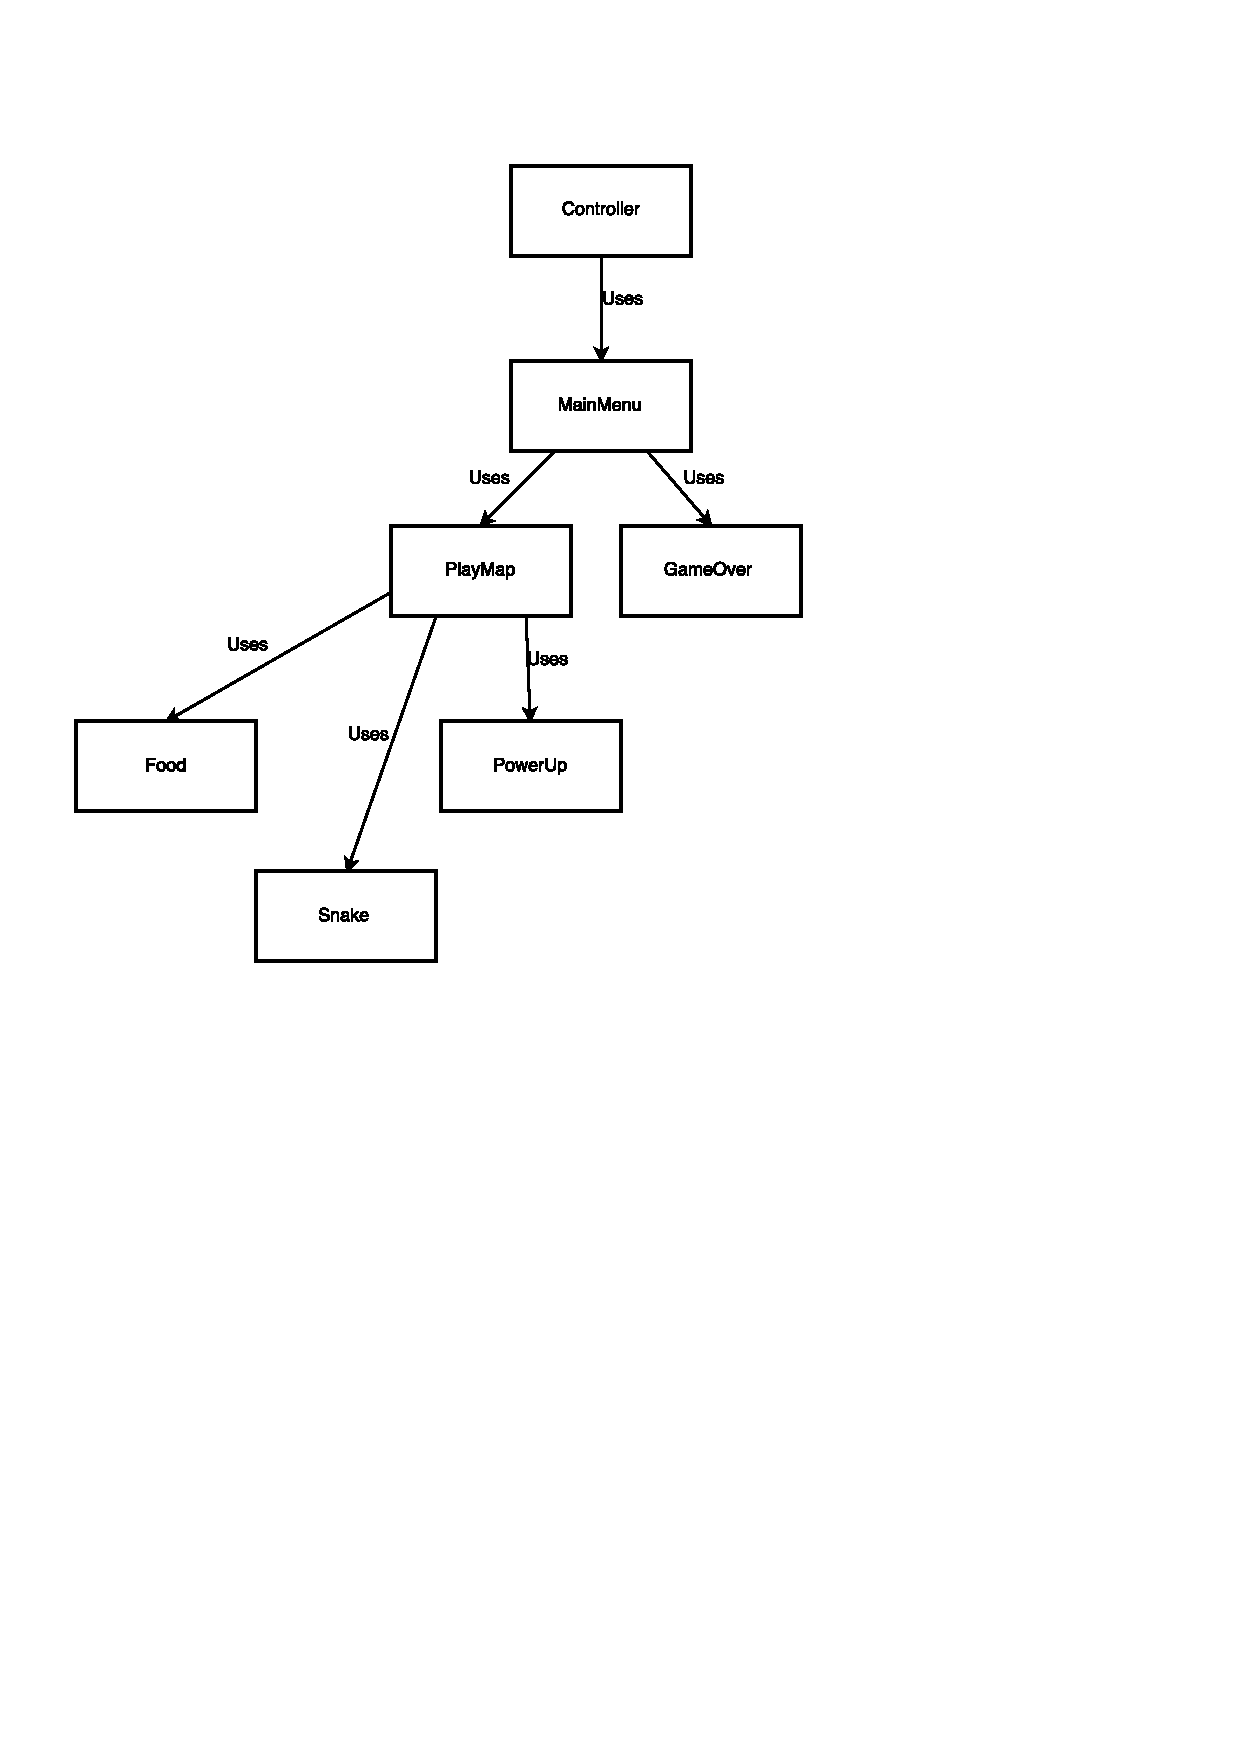
\includepdf[pages={1}]{UsesHeirarchy.pdf}



%\section*{References}

\bibliographystyle {plainnat}
\bibliography {../PCM_SRS/PCM_SRS}

\end{document}
